\section{Merging code changes from a branch to the master\label{sec:pull_requests}}

This section describes how to merge changes from a branch to the master repository. See the guidelines in Section~\ref{sec:buildrules} for more information on building \CNAME. 

\emph{Note:} When merging changes, check that the new code doesn't break any of the existing unit-tests or auto-differentiation code. You will need to build using the commands listed below before merging changes.

\begin{enumerate}
	\item \texttt{doBuild archive} this will build all the autodiff librarys.
	\item \texttt{doBuild modelrunner}
	\item Enter the directory  \texttt{BuildSystem\textbackslash Casal2\textbackslash Casal2 - -unittest} to check all the unit-tests pass.
\end{enumerate}

This section differs from Section~\ref{sec:maintain_repo} (where we pulled changes from the master repository into a branch). Here we are merging changes from a branch into the master, which will be incorporated into the master version of \CNAME. From this example we can see from Figure~\ref{fig:fork_merge1} that our branch is 109 commit ahead and 844 commits behind (underlined in blue) that we want to incorporate into the master repository.

To incorporate these changes into the master you need to click on the \enquote{pull request} button. This will prompt a comparison of the changes that you are submitting for inclusion into the master.

\begin{figure}[H]
	\centering
	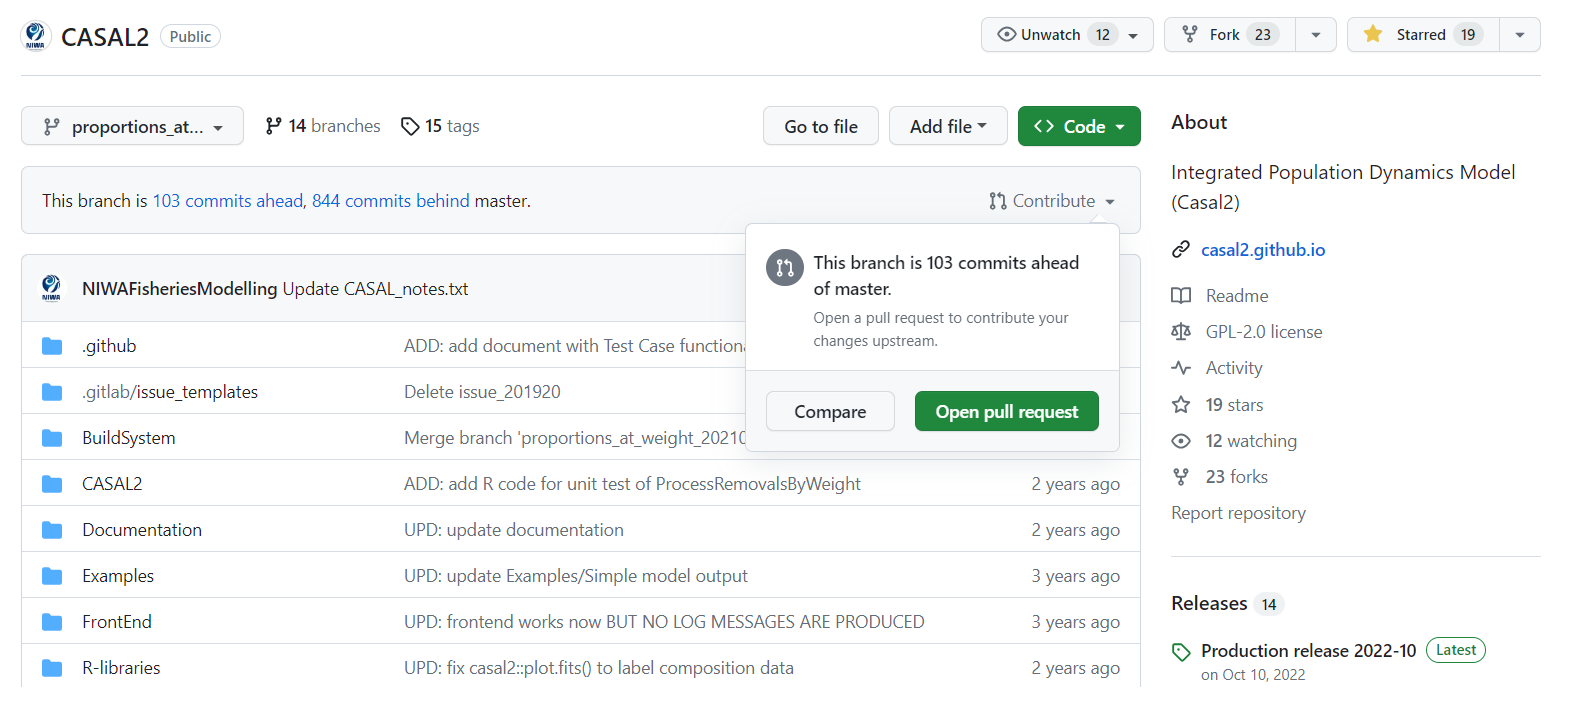
\includegraphics[scale=0.4]{Figures/create_pull_request.png}
	\caption{Example showing differences between a fork and the master in GitHub}\label{fig:fork_merge1}
\end{figure}

We can see that there are ten files changed from three commits. A the top left corner there is a green button with \enquote{create pull request} click that button. This will open a pull request on the master repository as shown in Figure~\ref{fig:fork_merge2}

\begin{figure}[H]
	\centering
	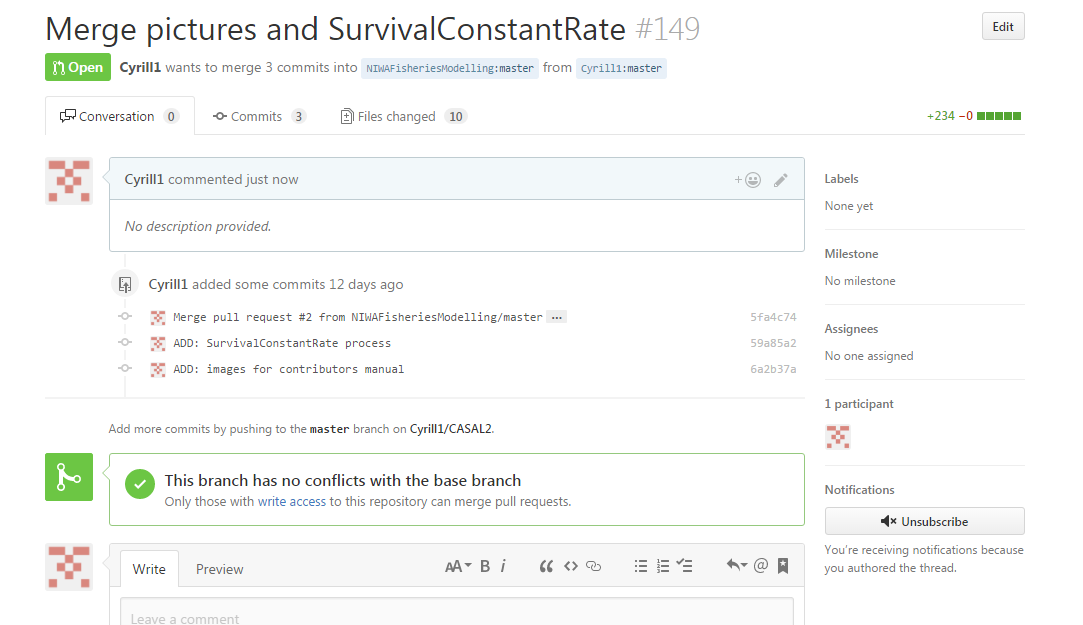
\includegraphics[scale=0.6]{Figures/Pull_request1.png}
	\caption{Example of a pull request in GitHub}\label{fig:fork_merge2}
\end{figure}

This will notify the maintainers of the master repository that a contributor is requesting a merge of the forked code into the master. Maintainers are able to look through the proposed code changed and will discuss the changes with the contributor if they need clarification. But at this point we are just waiting for the maintainers to accept the changes which then get incorporated into \CNAME.
